  \usepackage{amssymb}
  \usepackage{latexsym}
  \usepackage{amsfonts}
  \usepackage{amsthm}
  \usepackage{amsmath}


% put your command and environment definitions here

 \newcommand{\needscitation}[2]{\textcolor{red}{\textbf{#1} (from: #2)}}

 \newcommand{\red}[1]{\textcolor{red}{#1}}
 \newcommand{\TODO}{\textcolor{red}{TODO}}
 \newcommand{\todo}{\textcolor{red}{TODO}}

 \newcommand{\placeholderimage}{
  \begin{figure}[h!]
    \centering
    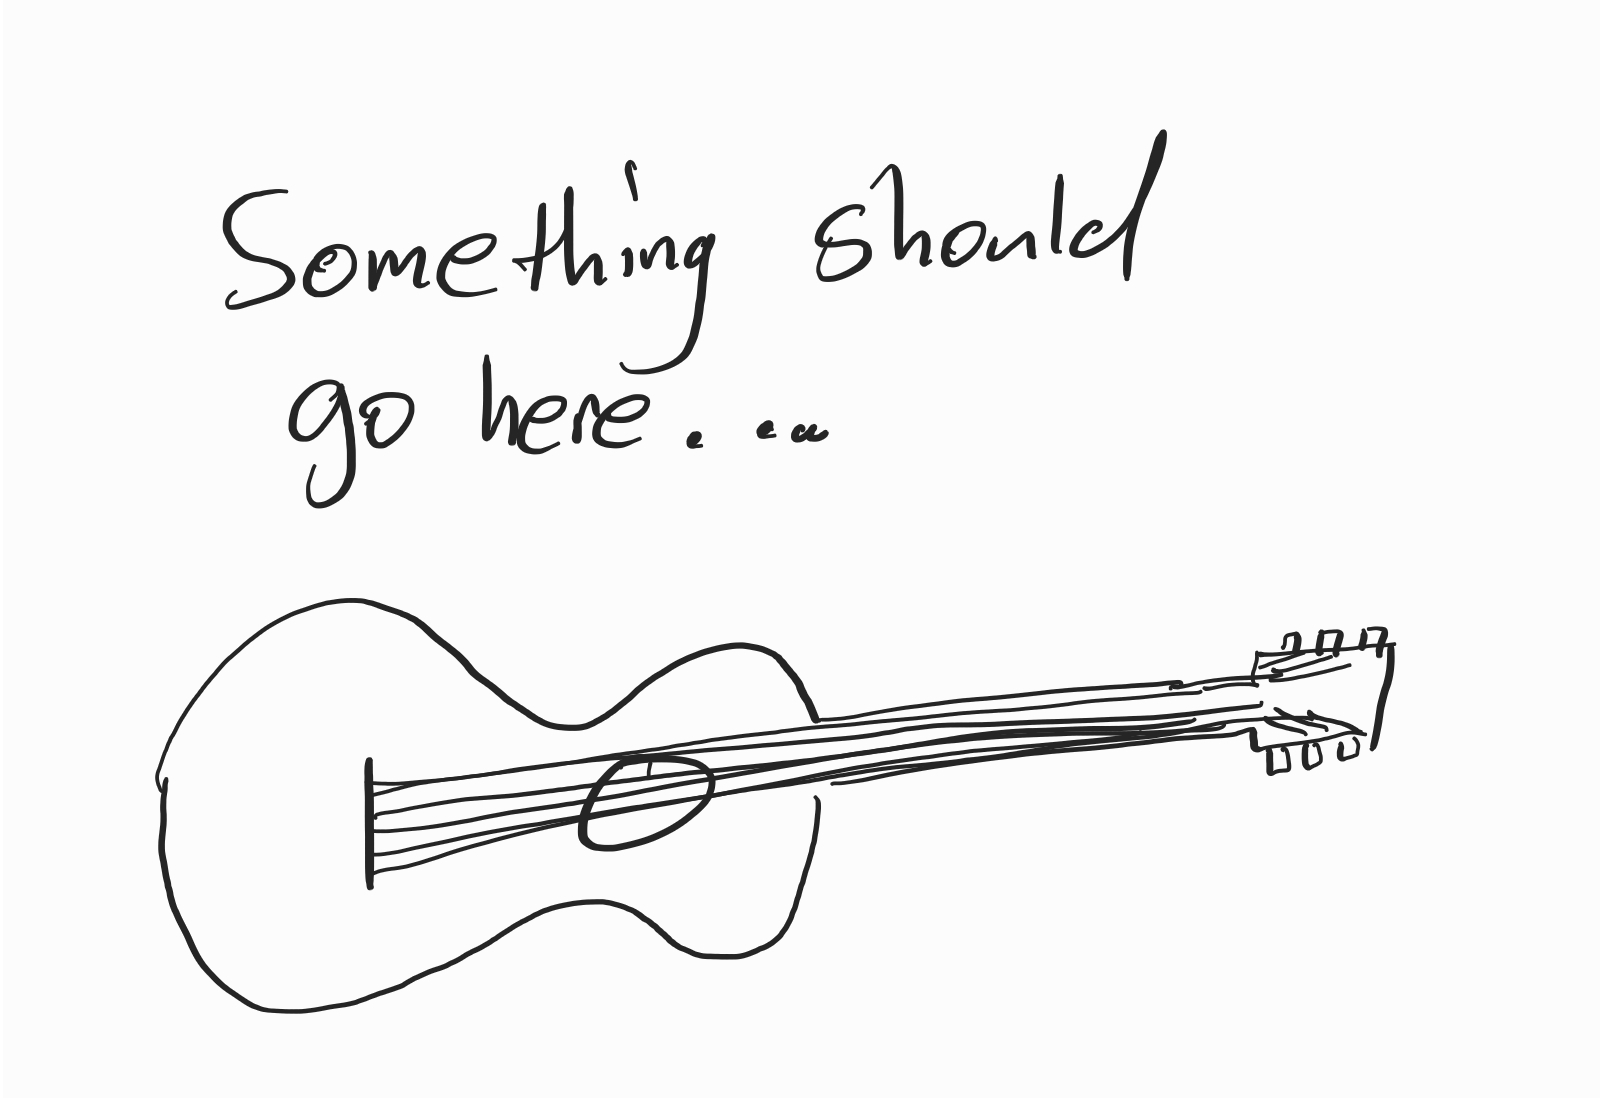
\includegraphics[scale=0.7]{imgs/placeholder.jpg}
    \caption{This should say something meaningful...}
  \end{figure}
 }



% Some theorem environments
% remove "[theorem]" if you do not want them to use the same number sequence


  \newtheorem{theorem}{Theorem}[chapter]
  \newtheorem{lemma}[theorem]{Lemma}
  \newtheorem{proposition}[theorem]{Proposition}
  \newtheorem{corollary}[theorem]{Corollary}

  \newtheorem{conj}{Conjecture}
  \renewcommand{\theconj}{\Alph{conj}}  % numbered A, B, C etc

  \theoremstyle{definition}
  \newtheorem{definition}[theorem]{Definition}
  \newtheorem{example}[theorem]{Example}
  \newtheorem{examples}[theorem]{Examples}
  \newtheorem{question}[theorem]{Question}
  \newtheorem{remark}[theorem]{Remark}
  \newtheorem{notn}[theorem]{Notation}

  
